\section{Software}

This section describes the various software tools used during the CLAS12 Trigger System development, validation, and operation.

\subsection{Development Software}

Several software packages were used to implement and test the trigger logic developed for CLAS12. These were the FPGA synthesis and implementation packages, and the FPGA high-level synthesizer.

For FPGA synthesis and implemenation, Xilinx ISE/Planahead and Vivado were used. Most of the front-end boards were developed years ago and use Virtex-5 and Spartan 6 FPGAs, which are not supported by Xilinx Vivado, so we relied on Xilinx ISE/Planahead for synthesis and implementation. Even though these tools are no longer updated by Xilinx, they have proved to be stable, reliable, and deliver consistent results. Newer designs use Xilinx 7-series parts (we used Artix, Kintex, and Virtex), so we used the Vivado tools, which had far better support than ISE/Planahead.

Vivado HLS was used to implement a variety of trigger algorithms, Event Builder logic, and general purpose logic. HLS components were able to be verified with C/C++ test benches on their own without anything more than GNU GCC and associated C/C++ header files from the HLS toolchain. This tool often allowed for faster FPGA implemenation, but many components still were implemented in HDL where resource and/or timing requirements become critical. Vivado HLS generated VHDL files from the C/C++ sources that were included into the FPGA compilation and full simulations. Occasionally simulation of the HDL-generated files was required to debug C/C++ modules when simulation under GCC found no problem, but the HDL result did. Differences between the C/C++ simulation and the corresponding HDL output were primarily due to: C/C++ assumption of infinite length buffering while HDL buffers were finite, ambiguous C/C++ coding where GCC and HLS behaviors differed, and latency issues due to the C/C++ simulation having no concept of elapsed time. Our experience with HLS is described in detail in Section \ref{sec:hls}.

\subsection{Operating Systems}

Linux operating systems are used on all readout controllers in the CLAS12 DAQ. The VME crate controllers use Intel-based CPUs and run a standard Centos and Linux kernel distribution. The VTP modules use an ARMv7 CPU with custom hardware and run Arch Linux using a custom Linux kernel. Both CPUs boot from the network using a shared kernel and root filesystem images, which simplifies administration. Common DAQ software (readout, configuration, slow control, diagnostics, etc.) tools are used for both platforms and most tools available on standard desktop PCs are also available.

Details on the installation of Arch Linux with ARMv7 are as following:

\begin{itemize}
\item Linux kernel 4.4.0
  \begin{itemize}
  \item Updates with specific support for Xilinx Zynq Processors
  \item Available at https://github.com/Xilinx/linux-xlnx.git
  \item Custom device-tree
  \item Provides FPGA programming interface
  \item Allocates physical memory for use with DMA and event buffers
  \item Standard I$^2c$ and SPI API
  \end{itemize}

\item Arch Linux compiled for ARMv7
  \begin{itemize}
  \item Available at https://archlinuxarm.org/
  \item Filesystem over NFS
  \item Diskless booting using tftp (UBoot)
  \end{itemize}
\end{itemize}


\subsection{Configuration Software}

\subsubsection{Configuration Files}

The CLAS12 Trigger System has a large number of parameters controlling its logic. Those parameters are set by writing values to hardware registers, and are controlled by reading those registers back. The system uses ASCII configuration files, as shown for example in (Fig.\ref{fig:config}). Every line in these configuration files contains a key word and the number of corresponding parameter values. The directive ``include'' can be used to create a hierarchical set of configuration files. Normally the main configuration file is selected during the run startup procedure, and the CLAS12 run control software resolves all ``include'' directives, resulting in the creation of one big configuration file. That file is used to program all trigger hardware registers, and its content is also written to the data stream for bookkeeping purposes. The register contents are read back and the results are recorded into the data stream as well, providing full control of the Trigger System settings. Normally the same configuration files contain the DAQ settings as well, making it a complete source for the entire DAQ/Trigger System settings.

\begin{figure}[hbt]
	\centering
	
\includegraphics[width=1.0\columnwidth,keepaspectratio]{img/config.png}
	\caption{Configuration file example. Flat text configuration files were used for all DAQ and trigger components. Download and Upload procedures were implemented, with uploaded settings being stored into data files and databases. The format used allows personnel with appropriate training to understand and modify the system settings using text editors. Version control is enforced using Github.}
	\label{fig:config}
\end{figure}


\subsubsection{Timing Settings}

\begin{figure}[hbt]
	\centering
	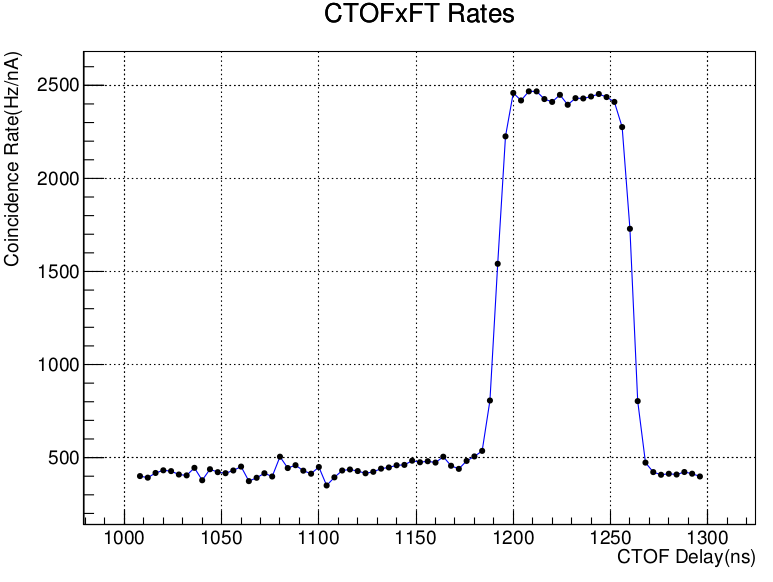
\includegraphics[width=1.0\columnwidth,keepaspectratio]{img/delay_scan_ctof_ft.png}
	\caption{CTOFxFT Delay Scan. In this scan the FT trigger time was fixed as having the smallest jitter, and the CTOF trigger delay was changed. Similar delay scans were measured for all detectors participating in the trigger logic, to make sure all trigger components were in time.}
	\label{fig:delay_scan_ctof_ft}
\end{figure}

One of the important aspects in setting up the trigger is the measurement of the relative timing between the signals from the detector elements used to define a trigger. These are referred to as delay curves. For this purpose software procedures were developed. This includes special trigger configuration files and software tools to scan individual subsystem latencies, record sets of beam current normalized scalers, and produce the corresponding delay plots (see Fig.~\ref{fig:delay_scan_ctof_ft}). The trigger time setting for a specific detector element was kept at a constant value, which determined the DAQ readout time window width and offset, while the timing for the other subsystems were changed step by step to monitor the delay curve. Delays and coincidence widths were adjusted to account for known jitter sources to ensure no events were lost due to poor timing alignment. This procedure was repeated every time the trigger logic was changed.


\subsubsection{Gain Calibration and Threshold Settings}

One of the important settings in the Trigger System is for the FADCs. As stated above, the FADC boards serve as the pre-trigger for most of the Stage 1 trigger components (except the Drift Chambers), and correct pedestal and gain calibrations for these units are critical for correct Trigger System performance. Pedestal and gain measurements are conducted before run startup, and the values are loaded using configuration files. All of the thresholds in the configuration files are set using physical units such as MeV for the calorimeter energy and the number of photoelectrons for the Cherenkov counter.


\subsection{Readout and Control Software}

All trigger hardware modules were implemented in VXS format and installed into VXS crates along with the other DAQ electronics. All readout and control libraries were developed as part of the DAQ System software project as described in Ref.~\cite{daq-ref}. From the software point of view, the DAQ and Trigger Systems can be considered as one system equipped with standard software tools.